% Provenance (never printed): see sources/outline_sources.md (Year 2: energy geology --- the
% petroleum system quantified, unconventional resources, geothermal systems, uranium deposits,
% geological storage of carbon dioxide).
% Kerogen kinetics and elemental analyses: Fletcher and Pugmire (DOE, OSTI 1176871); kerogen
% types and Easy%Ro: Advanced Chemistry Basins Project (DOE, OSTI 830009); maturity thresholds:
% USGS MF-2008-B; TTI: Waples (1980) and Hammerschmidt et al. (2014); volumetrics and CO2
% storage: DOE/NETL (2008) and IPCC SRCCS (2005) chapter 5; geothermal: USGS OFR 2008-1296 and
% FS 2008-3082; uranium: USGS Bulletin 1693; Oklo: OSTI abstract records. Ledger rows in
% sources/ledger/book4.md; curves from figdata/bachelor-2/maturation.py and co2_density.py,
% numbers from the Book 4 second-writer scratch calculator calc/ch30.py.
% Geology and sourced numbers only: no advocacy, no policy.
\chapter{ऊर्जा भूविज्ञान}\label{ch:b2:energy-geology}

तेल सूक्ष्म जीवों के अवशेष हैं, जो कीचड़ के साथ दबे और लगभग \qty{100}{\celsius} पर लाखों वर्षों तक
पकते रहे; भूतापीय ऊर्जा पृथ्वी की वही ऊष्मा है, जिसे सीधे लिया जाता है। दोनों तापमान और समय से शासित हैं:
पहली उस दर से जिससे कोई रासायनिक अभिक्रिया चलती है जब दबी हुई चट्टानें धीरे-धीरे गर्म होती हैं, दूसरी इस
बात से कि चट्टान का कोई आयतन कितनी ऊष्मा संचित करता है और जल उसे कितनी तेज़ी से किसी कुएँ तक ले जा सकता है।
यह अध्याय पेट्रोलियम तंत्र का परिमाणन करता है, फिर उन संसाधनों की ओर मुड़ता है जिनमें उसका कोई एक अवयव
नहीं होता, फिर भूतापीय ऊष्मा और यूरेनियम की ओर, और विपरीत क्रिया के साथ समाप्त होता है:
कार्बन डाइऑक्साइड को वापस भूमिगत रखना।
% ledger: earle:oil-window, earle:organic-preservation

\begin{recall}
\textbf{स्कूल की पुस्तकों से}: स्रोत चट्टान, केरोजन, परिपक्वन, तेल-खिड़की, प्रवासन,
भंडार चट्टान, आवरण चट्टान, ट्रैप, अधिभार, पेट्रोलियम तंत्र; कोयला और कोयले की कोटि; भूतापीय ऊर्जा।
\textbf{पुस्तक 3 (स्नातक वर्ष 1) से}: ऊष्मा-प्रवाह और भूतापीय वक्र; छिद्रता और पारगम्यता; छिद्र-द्रव
दाब, प्रभावी प्रतिबल और कूलॉम्ब कसौटी; बोरहोल लॉग; अवसादी द्रोणी और
अवधसान। \textbf{रसायन की पुस्तकों से}: आरेनियस नियम, सक्रियण ऊर्जा, प्रथम-कोटि
अभिक्रिया। \textbf{भौतिकी की पुस्तकों से}: रेडियोधर्मी क्षय, क्षय-नियतांक, अर्ध-आयु; किसी तरल का
क्रांतिक बिंदु। \textbf{\cref{ch:b2:basins-compared} से}: \omterm{def:b2:basins-compared:curve}{अवधसान वक्र}।
\textbf{\cref{ch:b2:ore-deposits} से}: \omterm{def:b2:ore-deposits:types}{अयस्क-निक्षेप प्रकार}, \omterm{def:b2:ore-deposits:grade}{टनभार}।
\end{recall}

\section{पेट्रोलियम तंत्र का परिमाणन}\label{sec:b2:energy-geology:petroleum}

किसी पेट्रोलियम तंत्र को केरोजन से समृद्ध एक स्रोत चट्टान, एक भंडार, एक आवरण चट्टान, एक ट्रैप और स्रोत
चट्टान को गर्म करने लायक़ पर्याप्त अधिभार चाहिए, और उसकी घटनाएँ सही क्रम में आनी चाहिए: जब तेल प्रवासन करे
तब ट्रैप का अस्तित्व होना चाहिए। उसके परिमाणन का अर्थ है तीन प्रश्नों का उत्तर देना: स्रोत चट्टान में किस प्रकार
का केरोजन है, उसका कितना रूपांतरण हो चुका है, और उत्पाद का कितना भाग ट्रैप में
स्थित है।
% ledger: magoon00:tps

\begin{definition}[केरोजन प्रकार, वान क्रेवेलेन आरेख]\label{def:b2:energy-geology:kerogen}
केरोजन अपने तत्त्वीय संघटन के अनुसार तीन \emph{केरोजन प्रकारों}\index{केरोजन प्रकार} में बँटते हैं:
प्रकार~I, सैप्रोपेलिक, हाइड्रोजन में सबसे समृद्ध, जो मुख्यतः तेल उत्पन्न करता है; प्रकार~III, ह्यूमिक या कोयलामय,
हाइड्रोजन में निर्धन, जो मुख्यतः मीथेन उत्पन्न करता है; और प्रकार~II, मध्यवर्ती, तेल और गैस दोनों का
स्रोत। \emph{वान क्रेवेलेन आरेख}\index{वान क्रेवेलेन आरेख} किसी केरोजन के परमाणु अनुपात H/C को
उसके परमाणु अनुपात O/C के विरुद्ध अंकित करता है; प्रकार उसके भिन्न क्षेत्रों में रहते हैं, और परिपक्वन
किसी केरोजन को निम्न H/C और निम्न O/C की ओर ले जाता है।
\end{definition}

एक प्रयोगशाला अध्ययन में विश्लेषित, ज्ञात प्रकार के सात अपरिपक्व केरोजनों का परमाणु H/C इस प्रकार है:
1.51 और 1.61 (प्रकार~I, जिनमें यूटा की ग्रीन रिवर तेल-शेल है, जो झीलों में निक्षेपित हुई और शैवालों के
अवशेषों से समृद्ध है), 1.22 से 1.28 (प्रकार~II, जिनमें उत्तरी सागर की किमरिज क्ले है),
1.13 (एक मिश्रित प्रकार~II/III) और 0.99 (प्रकार~III, कोलोराडो का कैमियो कोयला)। ग्रीन रिवर
केरोजन, द्रव्यमान से \qty{77}{\percent} कार्बन, औसतन C$_{100}$H$_{150}$N$_3$O$_8$S है: H/C 1.50 और
O/C 0.08। प्रयोगशाला में \qty{10}{K} प्रति मिनट पर गर्म करने पर यह एक अवशेष छोड़ता है जिसका H/C
\qty{460}{\celsius} पर 1.20 और \qty{525}{\celsius} पर 0.54 तक गिर जाता है, जबकि उसका O/C 0.08 से लगभग
0.01 तक गिरता है: नीचे के चित्र के बाईं ओर बना पथ।
% ledger: acb04:kerogens, fp14:gr-kerogen, fp14:gr-chars, mf88:thresholds
% values: GR3.9 kerogen H/C 1.486, O/C 0.080; chars 460 C 1.200/0.016, 525 C 0.544/0.011 (figdata maturation.py vk)

\begin{omfigure}
\centering
\begin{minipage}[b]{0.49\linewidth}\centering
\begin{tikzpicture}
\begin{axis}[omrecord, width=0.95\linewidth, height=5.0cm, xmin=0, xmax=0.12, ymin=0, ymax=1.8,
  xlabel={परमाणु O/C}, ylabel={परमाणु H/C}, xtick={0,0.04,0.08}, scaled x ticks=false,
  xticklabel style={/pgf/number format/fixed}, tick label style={font=\scriptsize},
  label style={font=\small}]
% computed in figdata/bachelor-2/maturation.py part vk; ledger: fp14:gr-kerogen, fp14:gr-chars
\addplot[omThm, line width=0.9pt, mark=*, mark size=1.3pt, -{Stealth[length=4pt]}] table[x=oc, y=hc] {figdata/out/bachelor-2-maturation-vk.dat};
\node[font=\scriptsize, text=omThm, anchor=north east] at (axis cs:0.081,1.45) {केरोजन};
\node[font=\scriptsize, text=omThm, anchor=west] at (axis cs:0.013,0.52) {\qty{525}{\celsius}};
% ledger: acb04:kerogens (H/C of immature kerogens; O/C not reported)
\draw[omThm, line width=1pt] (axis cs:0.104,1.51) -- (axis cs:0.12,1.51);
\draw[omThm, line width=1pt] (axis cs:0.104,1.61) -- (axis cs:0.12,1.61);
\draw[omProp, line width=1pt] (axis cs:0.104,1.22) -- (axis cs:0.12,1.22);
\draw[omProp, line width=1pt] (axis cs:0.104,1.25) -- (axis cs:0.12,1.25);
\draw[omProp, line width=1pt] (axis cs:0.104,1.28) -- (axis cs:0.12,1.28);
\draw[omExo, line width=1pt] (axis cs:0.104,1.13) -- (axis cs:0.12,1.13);
\draw[omDef, line width=1pt] (axis cs:0.104,0.99) -- (axis cs:0.12,0.99);
\node[font=\scriptsize, text=omThm, anchor=east] at (axis cs:0.103,1.58) {I};
\node[font=\scriptsize, text=omProp, anchor=east] at (axis cs:0.103,1.25) {II};
\node[font=\scriptsize, text=omDef, anchor=east] at (axis cs:0.103,0.97) {III};
\end{axis}
\end{tikzpicture}
\end{minipage}\hfill
\begin{minipage}[b]{0.49\linewidth}\centering
\begin{tikzpicture}
\begin{axis}[omrecord, width=0.95\linewidth, height=5.0cm, xmin=60, xmax=220, ymin=0, ymax=1,
  xlabel={तापमान (\unit{\celsius})}, ylabel={रूपांतरण अनुपात},
  tick label style={font=\scriptsize}, label style={font=\small}]
% computed in figdata/bachelor-2/maturation.py part tr; ledger: fp14:gr-daem
\addplot[black!40, densely dotted] coordinates {(60,0.5) (220,0.5)};
\addplot[omDef, line width=1.1pt] table[x=t_c, y=tr1] {figdata/out/bachelor-2-maturation-tr.dat};
\addplot[omThm, line width=1.1pt] table[x=t_c, y=tr10] {figdata/out/bachelor-2-maturation-tr.dat};
\addplot[omDef, line width=0.6pt, densely dashed] table[x=t_c, y=app1] {figdata/out/bachelor-2-maturation-tr.dat};
\addplot[omThm, line width=0.6pt, densely dashed] table[x=t_c, y=app10] {figdata/out/bachelor-2-maturation-tr.dat};
\node[font=\scriptsize, text=omDef, anchor=east] at (axis cs:125,0.80) {\qty{1}{\celsius\per\Myr}};
\node[font=\scriptsize, text=omThm, anchor=west] at (axis cs:160,0.30) {\qty{10}{\celsius\per\Myr}};
\end{axis}
\end{tikzpicture}
\end{minipage}
\par\smallskip{\small बाएँ: एक \omterm{def:b2:energy-geology:kerogen}{वान क्रेवेलेन आरेख}। लाल पथ ग्रीन रिवर प्रकार~I केरोजन और
\qty{10}{K} प्रति मिनट पर 400--\qty{525}{\celsius} तक प्रयोगशाला-तापन के बाद उसके अवशेषों का है;
दाईं ओर के चिह्न प्रकार~I (लाल), II (नारंगी), II/III (धूसर) और III (नीला) के सात अपरिपक्व केरोजनों
का H/C दर्शाते हैं, जिनका O/C दर्ज नहीं किया गया। डेटा: Fletcher और Pugmire (2014);
Advanced Chemistry Basins Project (2004)। दाएँ: \qty{10}{\celsius} से स्थिर दरों पर गर्म किए गए
ग्रीन रिवर केरोजन का रूपांतरण अनुपात, उसकी सक्रियण ऊर्जाओं के बंटन के साथ (ठोस) और केवल उसकी
माध्य ऊर्जा के साथ, \eqref{eq:b2:energy-geology:maturation} द्वारा (डैश)।}
\end{omfigure}

केरोजन का पेट्रोलियम में रूपांतरण प्रथम-कोटि अभिक्रियाओं का एक समुच्चय है, जिनमें से हर एक आरेनियस नियम
का पालन करती है। अवधसित होती द्रोणी में किसी स्रोत चट्टान का तापमान धीरे-धीरे और लगभग
स्थिर रूप से बढ़ता है, जिससे निम्नलिखित परिणाम परिपक्वन मॉडलों का केंद्र बन जाता है।

\begin{proposition}[स्थिर तापन-दर पर प्रथम-कोटि अभिक्रिया]\label{prop:b2:energy-geology:maturation}
मान लीजिए दर-नियतांक $k = A\,e^{-E/RT}$ वाली कोई प्रथम-कोटि अभिक्रिया ऐसे पदार्थ में चलती है जिसे
स्थिर दर $\beta = \mathrm{d}T/\mathrm{d}t$ से उस तापमान $T_0$ से गर्म किया जाता है जिस पर $k$ नगण्य है।
तापमान $T$ पर अरूपांतरित बचा अंश है
\begin{equation}
x(T) = \exp\Bigl[-\frac{A}{\beta}\int_{T_0}^{T} e^{-E/RT'}\,\mathrm{d}T'\Bigr]
\approx \exp\Bigl[-\frac{A R T^2}{\beta E}\,e^{-E/RT}\Bigr] ,
\label{eq:b2:energy-geology:maturation}
\end{equation}
सन्निकटन तब मान्य है जब $E/RT \gg 1$; रूपांतरण अनुपात $1 - x$ है।
\end{proposition}

\begin{proof}
प्रथम कोटि का अर्थ है $\mathrm{d}x/\mathrm{d}t = -k x$। $\mathrm{d}t = \mathrm{d}T/\beta$ के साथ
$\mathrm{d}\ln x = -(A/\beta)\,e^{-E/RT}\,\mathrm{d}T$, और $x = 1$ से, जो $T_0$ पर है, समाकलन करने पर
पहला रूप मिलता है। समाकल के लिए, $\frac{\mathrm{d}}{\mathrm{d}T}\bigl[\frac{RT^2}{E}e^{-E/RT}\bigr]
= \bigl(1 + \frac{2RT}{E}\bigr)e^{-E/RT}$, अतः समाकल $\frac{RT^2}{E}e^{-E/RT}$ के बराबर है, कोटि
$2RT/E$ के एक सापेक्ष संशोधन तक, और निचली सीमा का कोई योगदान नहीं होता क्योंकि $e^{-E/RT_0} \ll
e^{-E/RT}$।
\end{proof}

दो परिणाम निकलते हैं। रूपांतरण तापमान के एक संकीर्ण परास में होता है, क्योंकि
$e^{-E/RT}$ बहुत तेज़ी से बदलता है (अभ्यास~\ref{exo:b2:energy-geology:11})। और धीमा तापन निम्नतर
तापमान पर रूपांतरित करता है: $x = 1/2$ रखने पर, दस गुना तेज़ तापन-दर अर्ध-रूपांतरण का तापमान
लगभग $(RT^2/E)\ln 10$ बढ़ा देती है। प्रयोगशाला ताप-अपघटन पर समंजित ग्रीन रिवर केरोजन की गतिकी
$A = \qty{9.21e13}{s^{-1}}$ और $E/R = \qty{26800}{K}$ है ($E =
\qty{223}{kJ/mol}$); इस एकल ऊर्जा के साथ अर्ध-रूपांतरण \qty{136.4}{\celsius} पर होता है
\qty{1}{\celsius\per\Myr} के लिए, और \qty{150.9}{\celsius} पर \qty{10}{\celsius\per\Myr} के लिए: अंतर
\qty{14.5}{\celsius}, जबकि पूर्वानुमान $6.26 \times \ln 10 = \qty{14.4}{K}$ है।
\qty{10}{K} प्रति मिनट पर गर्म करने पर वही केरोजन \qty{450}{\celsius} के निकट रूपांतरित होता है
(अभ्यास~\ref{exo:b2:energy-geology:6}): समय तापमान का स्थान लेता है, इसीलिए गतिकी को लगभग 250 से
\qty{600}{\celsius} पर ताप-अपघटन द्वारा मापा जाता है, और इसीलिए तापन-दर में परिमाण की बारह कोटियों के पार
उसका बहिर्वेशन तेल-खिड़की की पूर्वानुमानित गहराई को अनिश्चित छोड़ देता है।
% ledger: fp14:gr-daem, acb04:kinetic-spread, codata:R
% values: Thalf 136.403 / 150.873 C; RT2/E 6.2587 K; lab 445.9 C (figdata maturation.py numbers, calc/ch30.py)

वास्तविक केरोजन में अनेक सामर्थ्यों के आबंध होते हैं, इसलिए उसकी गतिकी सक्रियण ऊर्जाओं का एक बंटन है, जिसका
हर अंश प्रतिज्ञप्ति का पालन करता है; ग्रीन रिवर केरोजन के लिए यह बंटन प्रसामान्य है, मानक विचलन
$\sigma/R = \qty{481}{K}$ के साथ। बंटन रूपांतरण को फैला देता है, जैसा चित्र का दायाँ भाग दिखाता है:
\qty{150}{\celsius} पर, \qty{1}{\celsius\per\Myr} पर गर्म किया गया केरोजन \qty{93}{\percent} रूपांतरित है,
और दस गुना तेज़ी से गर्म किया गया
\qty{48}{\percent}।
% ledger: fp14:gr-daem
% values: TR 0.927 / 0.484 at 150 C (figdata maturation.py numbers)

\begin{definition}[विट्रिनाइट परावर्तकता, समय--तापमान सूचकांक]\label{def:b2:energy-geology:maturity}
\emph{विट्रिनाइट परावर्तकता}\index{विट्रिनाइट परावर्तकता}, $R_o$, आपतित प्रकाश का वह प्रतिशत है जो
विट्रिनाइट के पॉलिश किए गए कणों से परावर्तित होता है --- विट्रिनाइट कोयले और केरोजन का एक कार्बनिक घटक है ---
और जिसे सूक्ष्मदर्शी के नीचे मापा जाता है; यह तापन के साथ अनुत्क्रमणीय रूप से बढ़ती है और किसी चट्टान द्वारा प्राप्त उच्चतम तापीय परिपक्वता को दर्ज करती है। लोपातिन का
\emph{समय--तापमान सूचकांक}\index{समय--तापमान सूचकांक} (TTI) योग
$\sum_n \Delta t_n\,2^n$ है, जो \qty{10}{\celsius} के उन अंतरालों पर लिया जाता है जिनसे कोई चट्टान गुज़री है,
जहाँ $\Delta t_n$ क्रमांक $n$ वाले अंतराल में बिताया गया समय है, मिलियन वर्षों में; $n = 0$
100 से \qty{110}{\celsius} के लिए, $n = 1$ 110 से \qty{120}{\celsius} के लिए, $n = -1$ 90 से
\qty{100}{\celsius} के लिए, इत्यादि।
\end{definition}

परावर्तकता के पैमाने पर, प्रकार~I और II केरोजनों से तेल-उत्पादन $R_o =
\qty{0.60}{\percent}$ के निकट आरंभ होता है; 1.20 से \qty{1.30}{\percent} से ऊपर तेल अस्थिर है और टूटकर
मीथेन बनता है; प्रकार~III \qty{0.73}{\percent} के निकट मीथेन देना आरंभ करता है, और गैस-उत्पादन लगभग
\qty{4.8}{\percent} तक चलता रहता है। मॉडल $R_o$ की गणना किसी केरोजन की तरह करते हैं: Easy\%Ro मॉडल
विट्रिनाइट को बीस समांतर प्रथम-कोटि अभिक्रियाएँ मानता है, $A = \qty{e13}{s^{-1}}$ और
34 से \qty{72}{kcal/mol} (142 से \qty{301}{kJ/mol}) तक की ऊर्जाओं के साथ, और उनके रूपांतरित अंश $F$ को,
जो अधिकतम 0.85 है, $R_o = \exp(-1.6 + 3.7F)$ पर प्रतिचित्रित करता है, जो 0.20 से \qty{4.7}{\percent} तक जाता है।
% ledger: mf88:thresholds, acb04:easyro, fp14:gr-chars

किसी द्रोणी के हर संस्तर-तल के अनुदिश परावर्तकता इसी प्रकार परिकलित की जाती है। नीचे के चित्र की काल्पनिक
द्रोणी में अवसाद \qty{100}{m} प्रति मिलियन वर्ष की दर से 100 से \qty{70}{\Ma} तक जमा हुआ,
फिर \qty{35}{m} प्रति मिलियन वर्ष की दर से, \qty{10}{\celsius} की सतह और
\qty{30}{\celsius\per\km} की स्थिर प्रवणता के नीचे। उसके सबसे पुराने संस्तर-तल ने $R_o = \qty{0.6}{\percent}$
\qty{67.6}{\Ma} पर, \qty{3080}{m} और \qty{102}{\celsius} पर, प्राप्त किया, और \qty{1.3}{\percent}
\qty{11.6}{\Ma} पर, \qty{5040}{m} और \qty{161}{\celsius} पर; अब वह \qty{5450}{m} और
\qty{173.5}{\celsius} पर, $R_o = \qty{1.54}{\percent}$ पर स्थित है। चूँकि भूतापीय वक्र स्थिर है, इसलिए
परावर्तकता-अग्रभाग लगभग समताप रेखाओं के अनुदिश चलते हैं, और तेल-उत्पादन का आरंभ
\qty{100}{\celsius} के निकट है, स्कूल की पुस्तकों के 60 से \qty{120}{\celsius} के भीतर।
% ledger: acb04:easyro, mf88:thresholds, earle:settings, earle:oil-window
% values: figdata maturation.py numbers (oldest_ro06_*, oldest_ro13_*, ro_oldest_now)

\begin{omfigure}
\centering
\begin{tikzpicture}
\begin{axis}[omrecord, width=0.86\linewidth, height=4.8cm, xmin=0, xmax=100, ymin=0, ymax=5.6,
  x dir=reverse, y dir=reverse, ylabel={गहराई (km)}, xticklabels={}, name=bh,
  tick label style={font=\scriptsize}, label style={font=\small}]
% computed in figdata/bachelor-2/maturation.py parts burial and fronts (invented basin)
\addplot[black!40, densely dashed] coordinates {(100,1.333) (0,1.333)};
\addplot[black!40, densely dashed] coordinates {(100,3.0) (0,3.0)};
\addplot[black!40, densely dashed] coordinates {(100,4.667) (0,4.667)};
\node[font=\tiny, text=black!60, anchor=south east, fill=white, inner sep=1pt] at (axis cs:1,1.333) {\qty{50}{\celsius}};
\node[font=\tiny, text=black!60, anchor=south east, fill=white, inner sep=1pt] at (axis cs:1,3.0) {\qty{100}{\celsius}};
\node[font=\tiny, text=black!60, anchor=south east, fill=white, inner sep=1pt] at (axis cs:1,4.667) {\qty{150}{\celsius}};
\addplot[black!70, line width=0.5pt, unbounded coords=jump] table[x=t_ma, y expr=\thisrow{d90}/1000] {figdata/out/bachelor-2-maturation-burial.dat};
\addplot[black!70, line width=0.5pt, unbounded coords=jump] table[x=t_ma, y expr=\thisrow{d80}/1000] {figdata/out/bachelor-2-maturation-burial.dat};
\addplot[black!70, line width=0.5pt, unbounded coords=jump] table[x=t_ma, y expr=\thisrow{d70}/1000] {figdata/out/bachelor-2-maturation-burial.dat};
\addplot[black!70, line width=0.5pt, unbounded coords=jump] table[x=t_ma, y expr=\thisrow{d60}/1000] {figdata/out/bachelor-2-maturation-burial.dat};
\addplot[black!70, line width=0.5pt, unbounded coords=jump] table[x=t_ma, y expr=\thisrow{d50}/1000] {figdata/out/bachelor-2-maturation-burial.dat};
\addplot[black!70, line width=0.5pt, unbounded coords=jump] table[x=t_ma, y expr=\thisrow{d40}/1000] {figdata/out/bachelor-2-maturation-burial.dat};
\addplot[black!70, line width=0.5pt, unbounded coords=jump] table[x=t_ma, y expr=\thisrow{d30}/1000] {figdata/out/bachelor-2-maturation-burial.dat};
\addplot[black!70, line width=0.5pt, unbounded coords=jump] table[x=t_ma, y expr=\thisrow{d20}/1000] {figdata/out/bachelor-2-maturation-burial.dat};
\addplot[black!70, line width=0.5pt, unbounded coords=jump] table[x=t_ma, y expr=\thisrow{d10}/1000] {figdata/out/bachelor-2-maturation-burial.dat};
\addplot[black, line width=1.1pt, unbounded coords=jump] table[x=t_ma, y expr=\thisrow{d100}/1000] {figdata/out/bachelor-2-maturation-burial.dat};
\addplot[omDef, line width=1.4pt, unbounded coords=jump] table[x=t_ma, y expr=\thisrow{z06}/1000] {figdata/out/bachelor-2-maturation-fronts.dat};
\addplot[omThm, line width=1.4pt, unbounded coords=jump] table[x=t_ma, y expr=\thisrow{z13}/1000] {figdata/out/bachelor-2-maturation-fronts.dat};
\node[font=\scriptsize, text=omDef, anchor=north, fill=white, inner sep=1pt] at (axis cs:40,3.05) {$R_o = \qty{0.6}{\percent}$};
\node[font=\scriptsize, text=omThm, anchor=north west, fill=white, inner sep=1pt] at (axis cs:9,5.10) {\qty{1.3}{\percent}};
\node[font=\scriptsize, anchor=north east, fill=white, inner sep=1pt] at (axis cs:58,4.75) {स्रोत चट्टान};
\end{axis}
\begin{axis}[at={(bh.south west)}, anchor=north west, yshift=-0.15cm, width=0.86\linewidth,
  height=2.9cm, xmin=0, xmax=100, ymin=0.4, ymax=6.6, x dir=reverse, y dir=reverse,
  xlabel={समय (\unit{\Ma})}, ytick={1,2,3,4,5,6},
  yticklabels={स्रोत चट्टान, भंडार चट्टान, आवरण चट्टान, अधिभार, ट्रैप-निर्माण, उत्पादन},
  tick label style={font=\tiny}, label style={font=\small}, axis line style={black!60},
  xtick={100,80,60,40,20,0}]
% schematic events chart of the same invented basin
\fill[omLithShale!80!black] (axis cs:100,0.75) rectangle (axis cs:96,1.25);
\fill[omLithSand!70!black] (axis cs:90,1.75) rectangle (axis cs:85,2.25);
\fill[omLithShale!80!black] (axis cs:85,2.75) rectangle (axis cs:80,3.25);
\fill[black!25] (axis cs:80,3.75) rectangle (axis cs:0,4.25);
\fill[omProp!70] (axis cs:75,4.75) rectangle (axis cs:70,5.25);
\fill[omDef!70] (axis cs:67.6,5.75) rectangle (axis cs:11.6,6.25);
\end{axis}
\end{tikzpicture}
\par\smallskip{\small ऊपर: एक काल्पनिक द्रोणी का दफ़न-इतिहास (काला: हर 10 मिलियन वर्ष में
निक्षेपित संस्तर-तल, मोटा वाला स्रोत चट्टान), समताप रेखाएँ (डैश), और वे गहराइयाँ जहाँ
Easy\%Ro \qty{0.6}{\percent} (नीला) और \qty{1.3}{\percent} (लाल) तक पहुँचता है। नीचे: उसका घटना-चार्ट;
स्रोत चट्टान में उत्पादन $R_o = \qty{0.6}{\percent}$ से \qty{1.3}{\percent} तक चलता है,
ट्रैप बनने के बाद।}
\end{omfigure}

TTI पुराना और अपेक्षाकृत स्थूल है। यह मानता है कि परिपक्वन की दर हर \qty{10}{\celsius} पर दोगुनी हो जाती है,
जैसा $E \approx \qty{82}{kJ/mol}$ वाला कोई आरेनियस नियम
\qty{100}{\celsius} के निकट करता है (अभ्यास~\ref{exo:b2:energy-geology:5}); उसके पैमाने पर वेपल्स ने तेल-उत्पादन
का आरंभ 15 के TTI पर, उसका शिखर 75 पर और उसका अंत 160 पर रखा।
% ledger: waples80:tti, hamm14:tti-table

\begin{method}[समय--तापमान सूचकांक की गणना]\label{met:b2:energy-geology:tti}
आँकड़े स्रोत चट्टान का दफ़न-इतिहास और भूतापीय वक्र हैं, जिसे स्थिर माना जाता है।
\begin{enumerate}
  \item \textbf{तापमान-पथ।} हर समय पर गहराई को तापमान में बदलिए: सतह का तापमान
        जमा प्रवणता गुणा गहराई।
  \item \textbf{अंतरालों में समय।} बिताया गया समय $\Delta t_n$ ज्ञात कीजिए, \qty{10}{\celsius} के
        हर अंतराल में; जहाँ तापन-दर $\beta$ स्थिर है, वहाँ $\Delta t_n = \qty{10}{\celsius}/\beta$।
  \item \textbf{योग।} गुणनफल $\Delta t_n\,2^n$ समय के क्रम में जोड़िए; तेल-उत्पादन का आरंभ, शिखर और
        अंत तब प्राप्त होते हैं जब चालू योग 15, 75 और 160 को पार करता है।
\end{enumerate}
\end{method}

द्रोणी-मॉडल रूपांतरण को रूपांतरण अनुपात के रूप में व्यक्त करते हैं: किसी स्रोत चट्टान की मूल हाइड्रोकार्बन-क्षमता
का वह अंश जो रूपांतरित हो चुका है। कैलिफ़ोर्निया की एक द्रोणी के एक मॉडल में स्रोत चट्टान से निष्कासन
\qty{10}{\percent} के अनुपात पर आरंभ होता, \qty{50}{\percent} पर शिखर पर पहुँचता और \qty{95}{\percent} पर
समाप्त होता माना गया। निष्कासित तेल, जो जल से हल्का है, ऊपर की ओर पारगम्य भंडार चट्टानों में प्रवासन करता है,
और वहाँ रुकता है जहाँ कोई आवरण चट्टान किसी ट्रैप को बंद करती है।
% ledger: peters08b4:tr, magoon00:tps, earle:migration-traps

\begin{proposition}[स्थानस्थ तेल]\label{prop:b2:energy-geology:volumetrics}
मान लीजिए किसी ट्रैप का क्षेत्रफल $A$ है और उसके भंडार की शुद्ध मोटाई $h$, छिद्रता $\phi$ और जल-संतृप्ति
$S_w$ है, और $B_o$ उसके तेल का संरचना आयतन गुणक है: तेल की किसी मात्रा द्वारा भंडार में घेरे गए आयतन
और सतह पर उसके आयतन का अनुपात। \emph{आरंभिक स्थानस्थ स्टॉक-टैंक
तेल}\index{आरंभिक स्थानस्थ स्टॉक-टैंक तेल}, अर्थात् सतह पर मापा गया तेल-आयतन, है
\begin{equation}
\mathrm{STOIIP} = \frac{A\,h\,\phi\,(1 - S_w)}{B_o} .
\label{eq:b2:energy-geology:stoiip}
\end{equation}
\end{proposition}

\begin{proof}
भंडार का स्थूल आयतन $Ah$ है और उसका छिद्र-आयतन $Ah\phi$; छिद्रों का एक अंश $1 - S_w$ तेल रखता है,
अतः भंडार में तेल $Ah\phi(1 - S_w)$ घेरता है, और सतह पर इसका $1/B_o$ गुना
आयतन।
\end{proof}

\begin{definition}[पुनर्प्राप्ति गुणक]\label{def:b2:energy-geology:volumetrics}
किसी भंडार का \emph{पुनर्प्राप्ति गुणक}\index{पुनर्प्राप्ति गुणक} आरंभिक स्थानस्थ तेल (या गैस) का वह अंश है
जो उसके जीवनकाल में उत्पादित होता है।
\end{definition}

प्राथमिक उत्पादन और जल-अंतःक्षेपण द्वारा द्वितीयक पुनर्प्राप्ति मिलकर प्रायः स्थानस्थ तेल का 30 से \qty{40}{\percent} निकाल लेते हैं; कार्बन
डाइऑक्साइड का अंतःक्षेपण 10 से \qty{15}{\percent} और निकालता है। \qty{10}{km^2} का एक ट्रैप, \qty{30}{m} शुद्ध
भंडार, छिद्रता 0.20, तेल-संतृप्ति 0.70 और $B_o = 1.2$ के साथ, \qty{3.5e7}{m^3} स्टॉक-टैंक तेल रखता है,
जिसमें से 1.05 से \qty{1.4e7}{m^3} उत्पादित होगा।
% ledger: netl08:oilgas

\section{अपारंपरिक संसाधन}\label{sec:b2:energy-geology:unconventional}

\begin{definition}[अपारंपरिक भंडार]\label{def:b2:energy-geology:unconventional}
\emph{अपारंपरिक भंडार}\index{अपारंपरिक भंडार} इतनी कम पारगम्यता वाली चट्टान है कि उसके सूक्ष्म छिद्रों
में रखा तेल या गैस कृत्रिम उद्दीपन के बिना किसी आर्थिक दर पर किसी कुएँ तक नहीं बह सकता; उसका उत्पादन उसके
अनुदिश क्षैतिज रूप से खोदे गए और द्रवचालित विधि से विभंजित किए गए कुओं से होता है। शेल तेल और शेल गैस
स्वयं स्रोत चट्टान में रहते हैं, टाइट गैस निम्न-पारगम्यता वाले बलुआ पत्थरों और
कार्बोनेटों में।
\end{definition}

इस प्रकार कोई अपारंपरिक प्ले एक स्रोत चट्टान है, या उसके पास की कोई चट्टान, जिसने अपने उत्पन्न किए का एक भाग
रोके रखा। उसमें कौन-सा उत्पाद है, यह उसकी परिपक्वता से तय होता है: तेल-खिड़की में स्थित शेल तेल रखती है,
और $R_o \approx \qty{1.3}{\percent}$ से आगे की शेल गैस। शेल गैस का बड़े पैमाने पर उत्पादन लगभग
2000 में टेक्सास की बार्नेट शेल में आरंभ हुआ, और 2005 से संयुक्त राज्य के गैस-उत्पादन की अधिकांश वृद्धि
शेल, बलुआ पत्थर, कार्बोनेट और अन्य टाइट शैलसमूहों में क्षैतिज वेधन और द्रवचालित विभंजन से आई है;
गैस कोयला संस्तरों से भी निकाली जाती है।
% ledger: eia:shale-gas, eia:gas-coalbed, mf88:thresholds

\section{भूतापीय ऊर्जा}\label{sec:b2:energy-geology:geothermal}

\begin{definition}[भूतापीय तंत्र, स्थानस्थ ऊष्मा, एन्थैल्पी वर्ग, EGS]\label{def:b2:energy-geology:geothermal}
\emph{भूतापीय तंत्र}\index{भूतापीय तंत्र} भूपर्पटी का एक ऐसा आयतन है जहाँ ऊष्मा,
पारगम्यता और जल एक साथ आते हैं, ताकि कुओं से गर्म जल या भाप निकाली जा सके। किसी भंडार की
\emph{स्थानस्थ ऊष्मा}\index{स्थानस्थ ऊष्मा} वह ऊष्मा है जो वह अपने तापमान से किसी संदर्भ तापमान तक ठंडा होने
में छोड़ेगा। \emph{उच्च-एन्थैल्पी संसाधन}\index{उच्च-एन्थैल्पी संसाधन}
लगभग \qty{150}{\celsius} से ऊपर का भूतापीय तंत्र है; \emph{निम्न-एन्थैल्पी
संसाधन}\index{निम्न-एन्थैल्पी संसाधन} लगभग \qty{90}{\celsius} से नीचे का; दोनों के बीच
संसाधन को मध्यम कहा जाता है। तीनों ऊष्मा के प्रत्यक्ष उपयोग के लिए उपयुक्त हैं, पर सामान्यतः केवल मध्यम
और उच्च वर्ग ही बिजली उत्पन्न कर सकते हैं। \emph{संवर्धित भूतापीय तंत्र}\index{संवर्धित भूतापीय तंत्र} (EGS)
कम प्राकृतिक पारगम्यता वाली गर्म चट्टान का एक पिंड है जिसमें अभियांत्रिकी द्वारा पारगम्यता बनाई जाती है, ताकि
उसमें से जल परिसंचारित किया जा सके और उसकी ऊष्मा पुनर्प्राप्त की जा सके।
\end{definition}
% ledger: usgs08g:classes, usgs08g:egs

\begin{proposition}[स्थानस्थ ऊष्मा और पुनर्प्राप्य शक्ति]\label{prop:b2:energy-geology:heat}
आयतन $V$, माध्य तापमान $T_R$ और आयतनिक ऊष्मा-धारिता $C$ (चट्टान और छिद्र-तरल
मिलाकर) वाला कोई भंडार संदर्भ तापमान $T_0$ से ऊपर यह ऊष्मा रखता है:
\begin{equation}
q_R = C\,V\,(T_R - T_0) .
\label{eq:b2:energy-geology:heat}
\end{equation}
यदि उसका एक अंश $R_g$ उत्पादन-काल $\tau$ में कूप-मुखों तक पहुँचता है, तो उत्पादित माध्य तापीय
शक्ति $P = R_g\,q_R/\tau$ है।
\end{proposition}

\begin{proof}
कोई आयतन $\mathrm{d}V$, तापमान $T$ पर, $C\,\mathrm{d}V\,(T - T_0)$ छोड़ता है, $T_0$ तक ठंडा होने में;
एकसमान $C$ के साथ पूरे भंडार पर योग करने से $C\,V\,(T_R - T_0)$ मिलता है, जहाँ $T_R$ माध्य
तापमान है। शक्ति पुनर्प्राप्त ऊष्मा को समय से भाग देने पर मिलती है।
\end{proof}

संसाधन-आकलन \qty{15}{\celsius} के संदर्भ के साथ इस आयतन-विधि का उपयोग करते हैं। \omterm{def:b2:energy-geology:volumetrics}{पुनर्प्राप्ति
गुणक} $R_g$ अनिश्चित भाग है: आरंभिक आकलनों ने 0 और 0.5 के बीच 0.25 लिया; विभंजित भंडारों से
उत्पादन लगभग 0.1 की ओर संकेत करता है, 0.05 और 0.2 के बीच। $C = \qty{2.5}{MJ.m^{-3}.K^{-1}}$ के साथ
(चट्टान-आधात्रियाँ 2 से \qty{3}{MJ.m^{-3}.K^{-1}} रखती हैं), $3 \times 4 \times
\qty{1}{km}$ का एक भंडार, \qty{220}{\celsius} पर, \qty{6.15e18}{J} रखता है; 30 वर्षों में $R_g = 0.1$ के साथ यह
\qty{650}{MW} की माध्य तापीय शक्ति देता है। पारंपरिक क्षेत्र प्रति वर्ग किलोमीटर क्षेत्र 10 से
\qty{20}{MW} बिजली उत्पन्न करते हैं।
% ledger: usgs08g:volume, delaney86b4:properties, usgs08g:egs
% values: 6.15e18 J; 6.15e17 J; 649.6 MW (calc/ch30.py)

प्राकृतिक भूतापीय तंत्रों को ऊष्मा जितनी ही पारगम्यता की आवश्यकता होती है। अधिकांश बड़े तंत्र विवर्तनिक
प्लेटों के किनारों के निकट, ज्वालामुखियों, धूममुखों, गर्म झरनों और गीज़रों के बीच स्थित हैं, और उनकी
पारगम्यता प्रायः सक्रिय भ्रंशन से खुली दरारों की होती है: गहराई पर गर्म हुआ भूजल उनसे होकर ऊपर उठता है,
और कुएँ विभंजित भंडार से जल निकालते हैं, जैसा नीचे के खंड-चित्र में है। किसी EGS को प्राकृतिक भंडार की आवश्यकता नहीं होती:
उसके कुएँ, लगभग \qty{5}{km} तक खोदे गए, ऐसी गर्म चट्टान तक पहुँचते हैं जिसकी पारगम्यता अभियांत्रिकी से बनाई जाती है, और
संयुक्त राज्य के 2008 के एक आकलन ने उसकी अनंतिम क्षमता \qty{517800}{MW} बिजली आँकी,
जबकि अभिनिर्धारित पारंपरिक तंत्रों से \qty{9057}{MW}।
% ledger: eia:geo-where, usgs08g:egs, usgs08g:volume

\begin{omfigure}
\centering
\begin{minipage}[b]{0.55\linewidth}\centering
\begin{tikzpicture}[x=0.95cm, y=0.82cm, font=\scriptsize]
% schematic, not to scale
\fill[omLithSand!60] (0,0) -- (7,0) -- (7,-3.6) -- (0,-3.6) -- cycle;
\fill[omProp!35] (1.2,-1.05) .. controls (2.6,-0.85) and (4.4,-0.85) .. (5.8,-1.05)
  -- (5.8,-2.3) .. controls (4.4,-2.5) and (2.6,-2.5) .. (1.2,-2.3) -- cycle;
\fill[omThm!70] (2.6,-3.6) .. controls (2.8,-2.8) and (4.2,-2.8) .. (4.4,-3.6) -- cycle;
\draw[black, line width=0.8pt] (0,0) -- (7,0);
\foreach \x in {1.6,2.4,3.2,4.0,4.8,5.4} {\draw[black!55] (\x,-1.1) -- (\x+0.35,-2.2);}
\draw[omDef, line width=0.9pt, -{Stealth[length=4pt]}] (0.4,-0.1) .. controls (0.5,-2) and (1,-3) .. (2.4,-3.2);
\draw[omDef, line width=0.9pt, -{Stealth[length=4pt]}] (6.6,-0.1) .. controls (6.5,-2) and (6,-3) .. (4.6,-3.2);
\draw[omThm, line width=0.9pt, -{Stealth[length=4pt]}] (3.5,-2.85) -- (3.5,-1.2);
\draw[omThm, line width=0.9pt, -{Stealth[length=4pt]}] (3.5,-1.0) .. controls (3.6,-0.6) .. (5.4,0.02);
\draw[black, line width=1.1pt] (2.9,0.25) -- (2.9,-1.6);
\draw[black, line width=1.1pt] (4.3,0.25) -- (4.3,-1.7);
\fill[black] (2.75,0.25) rectangle (3.05,0.45);
\fill[black] (4.15,0.25) rectangle (4.45,0.45);
\node[anchor=south] at (5.4,0.05) {गर्म झरना};
\node[anchor=south] at (2.9,0.45) {कुआँ};
\node[anchor=south] at (4.3,0.45) {कुआँ};
\node[text=omDef, anchor=north west] at (0.05,-2.35) {ठंडा};
\node[text=omDef, anchor=north west] at (0.05,-2.65) {पुनर्भरण};
\node[align=center, fill=omProp!20, inner sep=1pt] at (5.1,-1.62) {विभंजित\\भंडार};
\node[text=white] at (3.5,-3.35) {अंतर्वेधन};
\end{tikzpicture}
\end{minipage}\hfill
\begin{minipage}[b]{0.40\linewidth}\centering
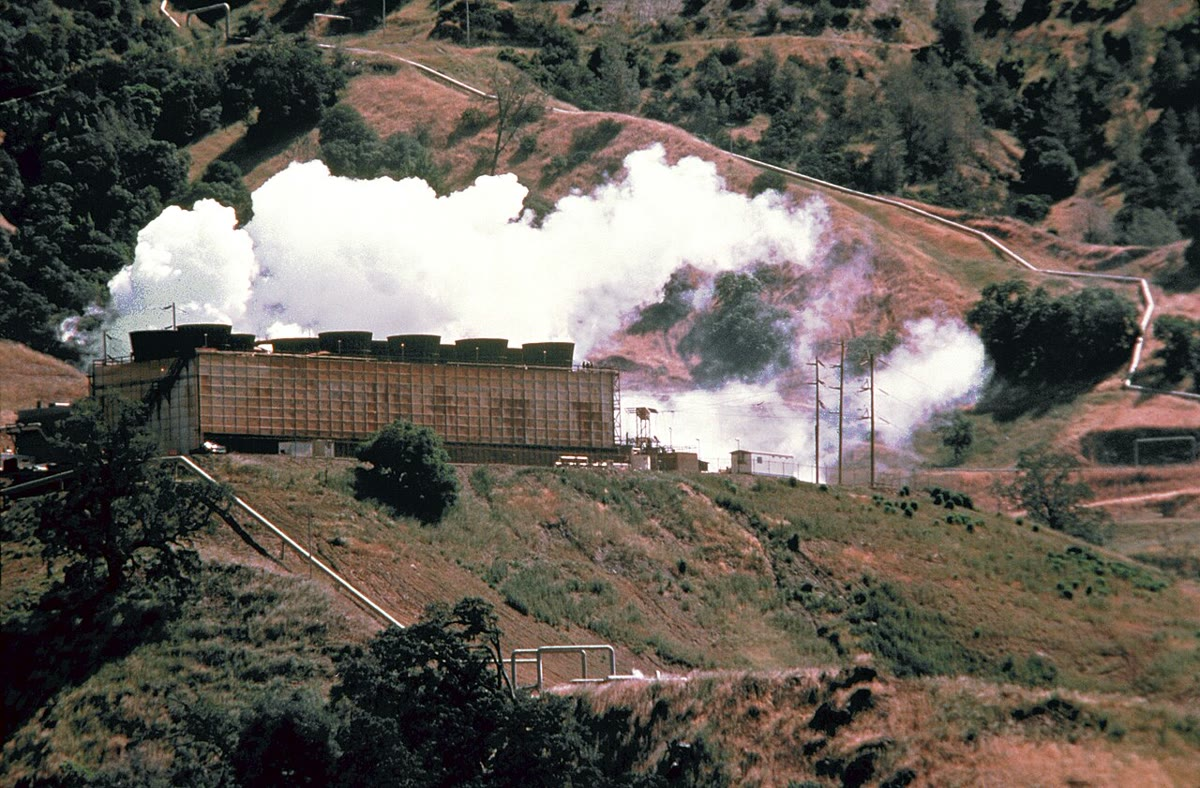
\includegraphics[width=\linewidth]{images/book4/b2-30-geyserville.jpg}
\end{minipage}
\par\smallskip{\small बाएँ: एक उच्च-एन्थैल्पी \omterm{def:b2:energy-geology:geothermal}{भूतापीय तंत्र} (योजनाचित्र, पैमाने पर नहीं): किनारों पर
पुनर्भरित जल (नीला) एक अंतर्वेधन के ऊपर गर्म होता है और एक विभंजित भंडार से होकर ऊपर उठता है
(लाल) एक गर्म झरने तक; कुएँ भंडार से जल निकालते हैं। दाएँ: गाइज़रविल, कैलिफ़ोर्निया के निकट
1982 में एक भूतापीय बिजलीघर, पहाड़ी ढलान पर भाप की पाइपलाइनों के साथ। फ़ोटो: U.S. Department of Defense
(सार्वजनिक डोमेन)।}
\end{omfigure}
% ledger: photo:b2-30-geyserville, usgs08g:egs

\begin{definition}[प्रेरित भूकंपनीयता]\label{def:b2:energy-geology:induced}
\emph{प्रेरित भूकंपनीयता}\index{प्रेरित भूकंपनीयता} मानवीय गतिविधियों से उत्पन्न भूकंपीय सक्रियता है जो
भूपर्पटी में प्रतिबल या छिद्र-द्रव दाब को बदलती हैं, प्रायः भूमि में तरल का
अंतःक्षेपण।
\end{definition}

तंत्र छिद्र-द्रव दाब सहित कूलॉम्ब कसौटी है: कोई भ्रंश तब सरकता है जब अपरूपण प्रतिबल
$\mu(\sigma_n - p)$ तक पहुँचता है, इसलिए $p$ बढ़ाने से पहले से प्रतिबलित भ्रंश विवर्तनिक भार में किसी परिवर्तन
के बिना विफलता की ओर बढ़ जाता है। 1960 के दशक में, डेनवर के निकट रॉकी माउंटेन आर्सेनल के नीचे विभंजित
प्रीकैम्ब्रियन आधार-चट्टान में 3.7 से
\qty{7.0}{km} की गहराइयों पर अंतःक्षेपित अपशिष्ट तरल ने भूकंप उत्पन्न किए; वे भंडार के उस भाग तक सीमित थे जहाँ
दाब \qty{32}{bar} (\qty{3.2}{MPa}) से अधिक बढ़ा था। ओक्लाहोमा के भूकंपों में तीव्र वृद्धि का कारण
अपशिष्ट जल का निपटान बताया गया है: चार उच्च-आयतन वाले
कुएँ मध्य संयुक्त राज्य की भूकंपनीयता के पाँचवें भाग के लिए उत्तरदायी हो सकते हैं, और वे
\qty{30}{km} से अधिक दूर भूकंप उत्पन्न करते हैं। किसी EGS भंडार का उद्दीपन छिद्र-दाब को
इसी प्रकार, जान-बूझकर, बढ़ाता है।
% ledger: hb81:denver, keranen:oklahoma, usgs08g:egs

\section{यूरेनियम}\label{sec:b2:energy-geology:uranium}

दो \omterm{def:b2:ore-deposits:types}{अयस्क-निक्षेप प्रकार} दिखाते हैं कि यूरेनियम कैसे सांद्रित होता है: एक किसी प्राचीन असंगति पर, दूसरा
बलुआ पत्थर में।

\begin{definition}[असंगति-संबद्ध और रोल-फ़्रंट यूरेनियम निक्षेप]\label{def:b2:energy-geology:uranium}
\emph{असंगति-संबद्ध यूरेनियम निक्षेप}\index{असंगति-संबद्ध यूरेनियम निक्षेप} पिचब्लेंड और यूरेनिनाइट का
एक पिंड है जो कायांतरित कार्बनमय पेलाइटों में और उनके ऊपर के क्वार्ट्ज़ एरेनाइटों में दरारें और ब्रेशिया भरता है,
किसी \omterm{def:b2:basins-compared:types}{अंतःक्रेटॉनिक द्रोणी} में आरंभिक और मध्य \omterm{def:b2:precambrian-earth:eons}{प्रोटेरोज़ोइक} चट्टानों के बीच की असंगति के नीचे, ऊपर या उसके
आर-पार। \emph{रोल-फ़्रंट यूरेनियम निक्षेप}\index{रोल-फ़्रंट यूरेनियम निक्षेप}
यूरेनियम खनिजों का एक अर्धचंद्राकार पिंड है जो किसी फ़ेल्डस्पारी या टफ़मय बलुआ पत्थर के संस्तरण को
ऑक्सीकृत और अपचयित भूमि की सीमा पर काटता है, जहाँ यूरेनियम एक स्थानीय रूप से अपचायी परिवेश में,
पायराइट के बीच, निक्षेपित हुआ।
\end{definition}

असंगति-निक्षेप 1800 से \qty{1200}{\Ma} की चट्टानों में स्थित हैं: असंगति के नीचे के कायांतरित
पेलाइट और उसके ऊपर के अकायांतरित बलुआ पत्थर; उनकी आतिथेय चट्टानें क्लोराइटीकृत हैं, और उनमें से अनेक के साथ मिलने वाले
ग्रेफ़ाइटी शिस्ट प्रबल विद्युत चालक हैं, जो विद्युत-चुंबकीय सर्वेक्षणों का लक्ष्य हैं। सस्कैचवान में की
लेक, क्लफ़ लेक और रैबिट लेक, और उत्तरी ऑस्ट्रेलिया में जाबिलुका और रेंजर इसके उदाहरण हैं। रोल-फ़्रंट अधिक युवा
हैं, अधिकतर तृतीयक: फ़ेल्सिक ज्वालामुखीय राख या ग्रेनाइट से पोषित बलुआ पत्थरों में, ऑक्सीकृत लौह खनिज
अग्रभाग से नति की ऊपरी दिशा में स्थित हैं और अपचयित खनिज नति की निचली दिशा में, जैसे वायोमिंग और टेक्सास
खाड़ी तट की द्रोणियों में।
% ledger: b1693:unconformity, b1693:sandstone

\begin{proposition}[अतीत में यूरेनियम-235]\label{prop:b2:energy-geology:u235}
मान लीजिए $r_0$ आज का परमाणु अनुपात $^{235}$U/$^{238}$U है और $\lambda_5$, $\lambda_8$ दोनों
समस्थानिकों के क्षय-नियतांक हैं। समय $t$ पहले यह अनुपात था
\begin{equation}
r(t) = r_0\,e^{(\lambda_5 - \lambda_8)\,t} ,
\label{eq:b2:energy-geology:u235}
\end{equation}
और यूरेनियम के परमाणुओं में $^{235}$U का अंश $r/(1 + r)$ था, $^{234}$U के अंश-मात्र की
उपेक्षा करते हुए।
\end{proposition}

\begin{proof}
हर समस्थानिक चरघातांकी रूप से क्षय होता है: $N_5(\text{अब}) = N_5(t)\,e^{-\lambda_5 t}$ और $N_8(\text{अब})
= N_8(t)\,e^{-\lambda_8 t}$। भाग देने पर $r_0 = r(t)\,e^{-(\lambda_5 - \lambda_8)t}$।
\end{proof}

$\lambda_5 = \qty{9.8485e-10}{yr^{-1}}$, $\lambda_8 = \qty{1.55125e-10}{yr^{-1}}$ और आज की
प्रचुरताओं \qty{0.7204}{\percent} और \qty{99.2742}{\percent} के साथ, $r_0 = 0.0072567$; \qty{2.0}{\Ga}
पहले $r = 0.0381$ था और प्राकृतिक यूरेनियम में \qty{3.67}{\percent} $^{235}$U था, जो आज के अंश का
पाँच गुना है।
% ledger: amherst:constants, iaea:isotopes
% values: r 0.038144, 3.6743 % (calc/ch30.py)

\begin{history}[दो अरब वर्ष पुराना एक रिएक्टर]
1972 में यूरेनियम अयस्क मापते हुए फ़्रांसीसी वैज्ञानिकों ने $^{235}$U की छोटी पर सार्थक कमियाँ पाईं, जिनका स्रोत
उन्होंने गैबॉन की ओक्लो खदान में खोजा। वहाँ चट्टान के पिंडकों में
\qty{65}{\percent} तक यूरेनियम था, जिसमें $^{235}$U का अंश सामान्य का आधा तक था, और ऐसा नियोडिमियम था
जो अपने आदिम समस्थानिक $^{142}$Nd में क्षीण पर 143 से 150 तक के उन समस्थानिकों में समृद्ध था जिन्हें विखंडन
उत्पन्न करता है: अयस्क में लगभग दो अरब वर्ष पहले शृंखला अभिक्रियाएँ चली थीं, लगभग \qty{300}{bar}
और 400 से \qty{500}{\celsius} पर। ऐसे सोलह प्राकृतिक रिएक्टर ओक्लो और पास के
बांगोम्बे में ज्ञात हैं, जो विश्व के वे एकमात्र दो निक्षेप हैं जहाँ ये पाए गए हैं; कार्बनिक पदार्थ ने यूरेनियम को
सांद्रित करने में सहायता की थी, और यूरेनियम ऑक्साइड ने तब से ऐक्टिनाइडों और
अवाष्पशील विखंडन-उत्पादों के अधिकांश भाग को अपनी जगह पर रोके रखा है।
\end{history}
% ledger: oklo:curtis, oklo:cowan, oklo:gl96, oklo:nagy

\section{कार्बन डाइऑक्साइड का भूवैज्ञानिक भंडारण}\label{sec:b2:energy-geology:ccs}

\begin{definition}[भूवैज्ञानिक \ce{CO2} भंडारण, प्रग्रहण क्रियाविधियाँ, भंडारण दक्षता गुणक]\label{def:b2:energy-geology:ccs}
\emph{भूवैज्ञानिक \ce{CO2} भंडारण}\index{भूवैज्ञानिक CO$_2$ भंडारण} कार्बन डाइऑक्साइड का गहरे
भूमिगत सरंध्र शैलसमूहों में --- क्षीण तेल और गैस भंडारों, गहरे लवणीय शैलसमूहों या कोयला संस्तरों में ---
लंबे समय तक रोके रखने के लिए अंतःक्षेपण है। उसे रोकने वाली \emph{\ce{CO2} प्रग्रहण
क्रियाविधियाँ}\index{CO$_2$ प्रग्रहण क्रियाविधियाँ} ये हैं: किसी आवरण चट्टान के नीचे संरचनात्मक (और स्तरिक)
प्रग्रहण; अवशिष्ट प्रग्रहण, केशिका बलों द्वारा छिद्रों में रोकी गई एक अचल प्रावस्था के रूप में;
विलेयता प्रग्रहण, शैलसमूह-जल में घुलकर; खनिज प्रग्रहण, खनिजों से अभिक्रिया करके कार्बोनेट बनने से;
और, कोयले और शेल में, कार्बनिक पदार्थ पर अधिशोषण। किसी शैलसमूह का \emph{भंडारण दक्षता गुणक}\index{भंडारण दक्षता गुणक}
$E$ उसके छिद्र-आयतन का वह अंश है जिसे अंतःक्षेपित
\ce{CO2} द्वारा भरे जाने की अपेक्षा की जा सकती है।
\end{definition}
% ledger: srccs:retention, netl08:saline

कार्बन डाइऑक्साइड सतह पर गैस है, पर उसका क्रांतिक बिंदु \qty{31.0}{\celsius} और
\qty{7.38}{MPa} पर है। \qty{25}{\celsius\per\km} के, \qty{15}{\celsius} से आरंभ होने वाले भूतापीय वक्र के अनुदिश,
द्रवस्थैतिक दाब के अधीन, तापमान \qty{641}{m} पर और दाब \qty{742}{m} पर क्रांतिक मान को पार करता है;
शुद्ध \ce{CO2} का घनत्व \qty{234}{kg.m^{-3}} (\qty{700}{m} पर) से उछलकर \qty{583}{kg.m^{-3}} (\qty{900}{m}
पर) हो जाता है, फिर 670 से \qty{700}{kg.m^{-3}} के निकट स्थिर हो जाता है, \qty{1.5}{km} से नीचे। एक टन
सतह पर \qty{534}{m^3} घेरता है और \qty{1.6}{m^3}, \qty{1000}{m} पर: 330 गुना कम; इसीलिए
भंडारण-आकलन केवल \qty{800}{m} से अधिक गहरे शैलसमूहों पर विचार
करते हैं।
% ledger: nist:co2-critical, data:b4-co2-density, srccs:density, netl08:saline
% values: z_tc 641.2 m, z_pc 742.2 m; volume ratio 331.9 (figdata co2_density.py numbers)

\begin{omfigure}
\centering
\begin{minipage}[b]{0.49\linewidth}\centering
\begin{tikzpicture}
\begin{axis}[omrecord, width=0.95\linewidth, height=5.2cm, xmin=0, xmax=750, ymin=0, ymax=3,
  y dir=reverse, xlabel={\ce{CO2} का घनत्व (\unit{kg.m^{-3}})}, ylabel={गहराई (km)},
  tick label style={font=\scriptsize}, label style={font=\small}]
% computed in figdata/bachelor-2/co2_density.py part profile; ledger: data:b4-co2-density
\addplot[black!45, densely dashed] coordinates {(0,0.742) (750,0.742)};
\node[font=\tiny, text=black!60, anchor=south east] at (axis cs:745,0.73) {क्रांतिक दाब};
\addplot[omDef, line width=1.1pt, mark=*, mark size=0.9pt] table[x=rho, y expr=\thisrow{depth_m}/1000] {figdata/out/bachelor-2-co2_density-profile.dat};
\end{axis}
\end{tikzpicture}
\end{minipage}\hfill
\begin{minipage}[b]{0.49\linewidth}\centering
\begin{tikzpicture}
\begin{axis}[width=0.95\linewidth, height=5.2cm, xmin=0, xmax=4, ymin=0, ymax=100,
  axis x line=bottom, axis y line=left, axis line style={-}, axis on top,
  xlabel={अंतःक्षेपण के बाद का समय (वर्ष)}, ylabel={भंडारित \ce{CO2} में हिस्सा},
  xtick={0,1,2,3,4}, xticklabels={1,10,100,1000,$10^4$}, ytick=\empty,
  tick label style={font=\scriptsize}, label style={font=\small}]
% schematic, after IPCC SRCCS (2005) Figure 5.9; ledger: srccs:trapping
% bands from the bottom: mineral, solubility, residual, structural (cumulative tops 0/0/1/5/15,
% 2/8/21/40/60, 10/30/56/80/90, 100)
\fill[omLithLime!60!black] (axis cs:0,0) -- (axis cs:1,0) -- (axis cs:2,1) -- (axis cs:3,5) -- (axis cs:4,15) -- (axis cs:4,0) -- cycle;
\fill[omDef!40] (axis cs:0,0) -- (axis cs:1,0) -- (axis cs:2,1) -- (axis cs:3,5) -- (axis cs:4,15) -- (axis cs:4,60) -- (axis cs:3,40) -- (axis cs:2,21) -- (axis cs:1,8) -- (axis cs:0,2) -- cycle;
\fill[omProp!40] (axis cs:0,2) -- (axis cs:1,8) -- (axis cs:2,21) -- (axis cs:3,40) -- (axis cs:4,60) -- (axis cs:4,90) -- (axis cs:3,80) -- (axis cs:2,56) -- (axis cs:1,30) -- (axis cs:0,10) -- cycle;
\fill[black!15] (axis cs:0,10) -- (axis cs:1,30) -- (axis cs:2,56) -- (axis cs:3,80) -- (axis cs:4,90) -- (axis cs:4,100) -- (axis cs:0,100) -- cycle;
\node[font=\scriptsize] at (axis cs:1.1,72) {संरचनात्मक};
\node[font=\scriptsize] at (axis cs:2.1,38) {अवशिष्ट};
\node[font=\scriptsize] at (axis cs:3.1,22) {विलेयता};
\node[font=\scriptsize, text=white, anchor=south east] at (axis cs:3.98,0.5) {खनिज};
\end{axis}
\end{tikzpicture}
\end{minipage}
\par\smallskip{\small बाएँ: \qty{25}{\celsius\per\km} के भूतापीय वक्र के अनुदिश, \qty{15}{\celsius} से आरंभ करके,
द्रवस्थैतिक दाब के अधीन, गहराई के साथ शुद्ध \ce{CO2} का घनत्व। डेटा: NIST Chemistry
WebBook (Span--Wagner अवस्था-समीकरण), कार्बन डाइऑक्साइड अभिग्रहण और भंडारण पर IPCC की विशेष रिपोर्ट (2005)
की परिस्थितियों के अनुदिश। दाएँ: समय के साथ प्रग्रहण क्रियाविधियाँ भंडारित \ce{CO2} को कैसे बाँटती हैं
(योजनाचित्र, उसी रिपोर्ट के आधार पर): आवरण चट्टान द्वारा प्रग्रहण अवशिष्ट, घुले हुए और खनिज रूपों को स्थान
देता है, जो कम गतिशील हैं।}
\end{omfigure}

\begin{proposition}[किसी शैलसमूह की भंडारण-क्षमता]\label{prop:b2:energy-geology:capacity}
क्षेत्रफल $A$, मोटाई $h$ और छिद्रता $\phi$ वाला कोई शैलसमूह, जिसमें \ce{CO2} का घनत्व $\rho$
है और \omterm{def:b2:energy-geology:ccs}{भंडारण दक्षता गुणक} $E$ है, यह द्रव्यमान भंडारित कर सकता है:
\begin{equation}
M = A\,h\,\phi\,\rho\,E .
\label{eq:b2:energy-geology:capacity}
\end{equation}
किसी क्षीण तेल-क्षेत्र के लिए, जिसने स्टॉक-टैंक आयतन $N_p$ उत्पादित किया है, उत्पादित तेल का आयतन-दर-आयतन
प्रतिस्थापन $M = \rho\,N_p\,B_o$ देता है।
\end{proposition}

\begin{proof}
छिद्र-आयतन $Ah\phi$ है, जिसके एक अंश $E$ को \ce{CO2} घनत्व $\rho$ पर भरती है। तेल-क्षेत्र में
उत्पादित तेल भंडार में $N_pB_o$ घेरता था, वही आयतन जिसे \ce{CO2} ले लेती है।
\end{proof}

गहरे लवणीय शैलसमूहों के लिए अनुकरण $E$ को छिद्र-आयतन के 1 से \qty{4}{\percent} के बीच देते हैं,
15 से 85 प्रतिशत के विश्वास-परास पर, लगभग \qty{2}{\percent} की माध्यिका के साथ: अधिकांश छिद्र-स्थान तक
कभी पहुँचा नहीं जाता, या वह अपना जल बनाए रखता है। \qty{1000}{km^2} का, \qty{50}{m} मोटा और
0.20 छिद्रता वाला एक शैलसमूह, \qty{2000}{m} पर ($\rho = \qty{686}{kg.m^{-3}}$), \qty{137}{Mt} भंडारित करता है, $E =
\qty{2}{\percent}$ पर।
% ledger: netl08:saline, data:b4-co2-density
% values: 1e9*50*0.2*686*0.02 = 1.372e11 kg (calc/ch30.py)

अंतःक्षेपित होने के बाद \ce{CO2} आवरण चट्टान के नीचे ऊपर उठती है और फैलती है। प्रवासन करते प्लूम के पीछे केशिका
बल अवशिष्ट संतृप्तियाँ रोके रखते हैं, जो छिद्र-स्थान के 15 से \qty{25}{\percent} तक पहुँच सकती हैं;
विलयन शैलसमूह-जल के प्रति घन मीटर 20 से \qty{60}{kg} \ce{CO2} ग्रहण करता है, और धीमे बहाव वाले
शैलसमूहों में अंतःक्षेपित \ce{CO2} का \qty{30}{\percent} तक दसियों वर्षों के भीतर घुल जाता है। विलेयता प्रग्रहण
दसियों से सैकड़ों वर्षों तक प्रधान रहता है, आयनिक रूप सैकड़ों से हज़ारों वर्षों तक, खनिज प्रग्रहण हज़ारों से
लाखों वर्षों तक: कार्बोनेट खनिजों के साथ अभिक्रियाओं में दिन लगते हैं, सिलिकेटों के साथ सैकड़ों से हज़ारों वर्ष।
भंडारण आयु के साथ अधिक सुरक्षित होता जाता है, और भली-भाँति चुने गए और भली-भाँति प्रबंधित स्थलों पर
1000 वर्षों में \ce{CO2} के \qty{99}{\percent} या अधिक भाग के रुके रहने को संभावित
माना गया।
% ledger: srccs:trapping, srccs:retention

\begin{dated}{2005}
उत्तरी सागर में, नॉर्वे से लगभग \qty{250}{km} दूर, स्लाइपनर में क्षेत्र की प्राकृतिक गैस से अलग की गई \ce{CO2},
जो उसका लगभग \qty{9}{\percent} है, अक्टूबर 1996 से उत्सिरा शैलसमूह में अंतःक्षेपित की जा रही है, जो
समुद्र-तल से 800 से \qty{1000}{m} नीचे एक असंपिंडित लवणीय बलुआ पत्थर है, लगभग \qty{1}{Mt} प्रति वर्ष की दर से।
2005 के आरंभ तक \qty{7}{Mt} से अधिक भंडारित हो चुकी थी, परियोजना के जीवनकाल में नियोजित \qty{20}{Mt} में से।
बार-बार किए गए भूकंपीय सर्वेक्षण प्लूम का प्रतिबिंब बनाते हैं, जिसका पदचिह्न तब लगभग \qty{5}{km^2} था, और
दिखाते हैं कि उसके ऊपर की आवरण चट्टान उसे बंद रखती है।
\end{dated}
% ledger: srccs:sleipner

\begin{inthefield}[खोदे जाते समय किसी कुएँ को पढ़ना]
\centering
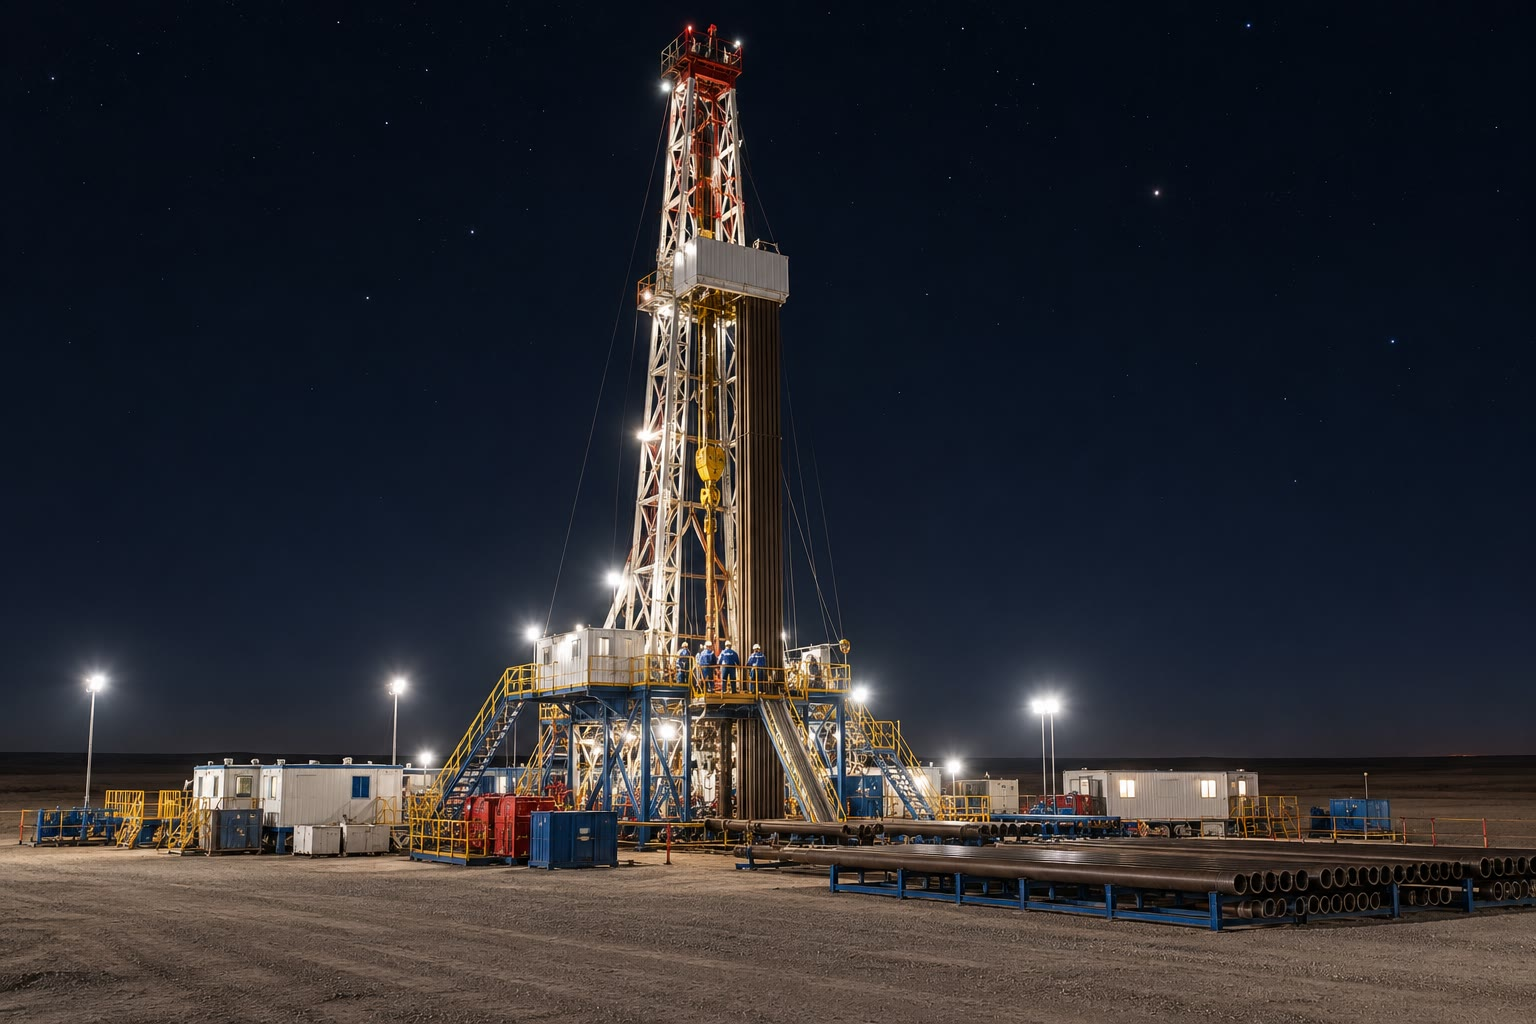
\includegraphics[width=0.56\linewidth]{images/book4/ai/b2-rig-night.jpg}
\par\smallskip{\small रात में एक स्थलीय वेधन-रिग (AI से बनाया गया चित्रण)।}
\par\medskip\raggedright
जब किसी कुएँ का कोई खंड पूरा हो जाता है, तो भूभौतिकीविद् एक केबल पर उपकरण नीचे उतारते हैं और गहराई के
सापेक्ष छिद्र के आसपास की चट्टानों के गुण दर्ज करते हैं। एक उपकरण उनकी प्राकृतिक रेडियोधर्मिता दर्ज करता है, जो
बलुआ पत्थर में कम और शेल में अधिक होती है; दूसरा उनका स्थूल घनत्व, जिससे छिद्रता इस प्रकार निकलती है:
(कण घनत्व $-$ स्थूल घनत्व)/(कण घनत्व $-$ तरल घनत्व), क्वार्ट्ज़ कणों के लिए \qty{2.65}{g/cm^3} और
जल के लिए लगभग \qty{1}{g/cm^3} के साथ। साथ पढ़े जाने पर ये बोरहोल लॉग भंडार की शुद्ध मोटाई और
वह छिद्रता देते हैं जो इस अध्याय के आयतनिक सूत्रों में प्रवेश करती हैं।
\end{inthefield}
% ledger: keys:gamma, keys:density-porosity

\section*{अभ्यास}\label{sec:b2:energy-geology:exercises}

अभ्यासों के आँकड़े, अन्यथा न कहा जाए तो: $R = \qty{8.314}{J.mol^{-1}.K^{-1}}$; एक मिलियन
वर्ष \qty{3.156e13}{s} है; ग्रीन रिवर केरोजन $A = \qty{9.21e13}{s^{-1}}$, $E/R = \qty{26800}{K}$;
परमाणु द्रव्यमान C 12.011, H 1.008, O 15.999; चित्र के प्रोफ़ाइल के अनुदिश \ce{CO2} का घनत्व:
सतह पर \qty{1.872}{kg.m^{-3}}, \qty{900}{m} पर 583, \qty{1000}{m} पर 621, \qty{2000}{m} पर
686। तीन सार्थक अंकों तक पूर्णांकित कीजिए।
% ledger: codata:R, fp14:gr-daem, data:b4-co2-density

\begin{exercise}[$\star$]\label{exo:b2:energy-geology:1}
(क)~चार अपरिपक्व केरोजनों का परमाणु H/C 1.58, 0.95, 1.24 और 1.12 है। हर एक को एक प्रकार दीजिए और बताइए
कि कौन मुख्यतः गैस देगा। (ख)~सूत्र C$_{100}$H$_{150}$N$_3$O$_8$S के अनुपात H/C और O/C
की जाँच कीजिए। (ग)~द्रव्यमान-संघटन C \qty{77.4}{\percent}, H
\qty{9.8}{\percent}, O \qty{8.2}{\percent} से उन्हें ज्ञात कीजिए।
\end{exercise}

\begin{exercise}[$\star$]\label{exo:b2:energy-geology:2}
(क)~प्रकार~II की एक स्रोत चट्टान के पाँच नमूनों का $R_o$ = 0.45, 0.68, 1.1, 1.6 और \qty{2.5}{\percent} है।
तेल और गैस के संदर्भ में हर एक की अवस्था का वर्णन कीजिए। (ख)~क्या $R_o =
\qty{0.68}{\percent}$ पर प्रकार~III का केरोजन मीथेन उत्पन्न कर रहा है? (ग)~Easy\%Ro का कौन-सा रूपांतरित अंश $F$
$R_o = 0.6$ और \qty{1.3}{\percent} के संगत है?
\end{exercise}

\begin{exercise}[$\star$]\label{exo:b2:energy-geology:3}
एक ट्रैप \qty{6}{km^2} क्षेत्र घेरता है; उसके भंडार की शुद्ध मोटाई \qty{25}{m}, छिद्रता 0.18 और जल-संतृप्ति
0.30 है, और $B_o = 1.25$। (क)~भंडार में तेल का आयतन और STOIIP ज्ञात कीजिए। (ख)~0.30 और 0.40 के
पुनर्प्राप्ति गुणकों के लिए उत्पादित आयतन ज्ञात कीजिए।
\end{exercise}

\begin{exercise}[$\star$]\label{exo:b2:energy-geology:4}
\qty{200}{m} मोटा एक बलुआ पत्थर जलभृत, \qty{10}{km^2} के नीचे, \qty{75}{\celsius} पर है। (क)~\qty{15}{\celsius} से ऊपर
उसकी \omterm{def:b2:energy-geology:geothermal}{स्थानस्थ ऊष्मा} ज्ञात कीजिए, $C = \qty{2.5}{MJ.m^{-3}.K^{-1}}$ के साथ। (ख)~वह किस
एन्थैल्पी वर्ग का है? (ग)~$R_g = 0.25$ के लिए 30 वर्षों में माध्य तापीय शक्ति ज्ञात कीजिए।
\end{exercise}

\begin{exercise}[$\star\star$]\label{exo:b2:energy-geology:5}
(क)~वह सक्रियण ऊर्जा ज्ञात कीजिए जिसके लिए कोई आरेनियस दर 100 और
\qty{110}{\celsius} के बीच दोगुनी हो जाती है। (ख)~उसी अंतराल में ग्रीन रिवर अभिक्रिया की दर किस गुणक से बढ़ती है?
(ग)~दोनों में से कौन-सा नियम किसी चट्टान द्वारा निम्न तापमान पर बिताए गए समय को अधिक भार देता है,
और प्रकार~I की स्रोत चट्टान के लिए परिकलित TTI के लिए इसका क्या अर्थ है?
\end{exercise}

\begin{exercise}[$\star\star$]\label{exo:b2:energy-geology:6}
(क)~\eqref{eq:b2:energy-geology:maturation} से दिखाइए कि अर्ध-रूपांतरण का तापमान
$T = (E/R)\big/\ln\bigl[A T^2/(\beta\,(E/R)\ln 2)\bigr]$ का पालन करता है, और \qty{1}{\celsius\per\Myr} पर तथा
\qty{10}{K} प्रति मिनट पर गर्म किए गए ग्रीन रिवर केरोजन के लिए इसे पुनरावृत्ति से हल कीजिए। (ख)~इस अंतर की
निम्नतर तापमान पर लिए गए अनुमान $(RT^2/E)\ln(\beta_2/\beta_1)$ से तुलना कीजिए, और
विसंगति को समझाइए।
\end{exercise}

\begin{exercise}[$\star\star$]\label{exo:b2:energy-geology:7}
\eqref{eq:b2:energy-geology:u235} और पाठ के आँकड़ों का उपयोग करके: (क)~प्राकृतिक यूरेनियम में $^{235}$U का अंश
\qty{2.0}{\Ga} और \qty{1.8}{\Ga} पहले ज्ञात कीजिए; (ख)~यह \qty{3.00}{\percent} कब था?
(ग)~ओक्लो अयस्क में $^{235}$U का अंश आज के सामान्य अंश का आधा तक है। उपभुक्त $^{238}$U की उपेक्षा करते हुए,
अभिक्रियाओं के समय उपस्थित $^{235}$U का कितना अंश विखंडित हुआ, और बाद का क्षय उत्तर को
क्यों नहीं बदलता?
\end{exercise}

\begin{exercise}[$\star\star$]\label{exo:b2:energy-geology:8}
(क)~\qty{1}{Mt} \ce{CO2} का आयतन सतह पर, \qty{1000}{m} पर और \qty{2000}{m} पर ज्ञात कीजिए। (ख)~स्लाइपनर में
2005 तक \qty{7}{Mt} से अधिक अंतःक्षेपित की जा चुकी थी, लगभग \qty{900}{m} पर, \qty{5}{km^2} पदचिह्न वाले एक प्लूम
में। प्लूम में छिद्रता 0.35 और \ce{CO2}-संतृप्ति 0.30 लेकर, उसके द्वारा घेरी गई चट्टान का आयतन और उसकी
माध्य मोटाई ज्ञात कीजिए।
\end{exercise}

\begin{exercise}[$\star\star$]\label{exo:b2:energy-geology:9}
एक उच्च-एन्थैल्पी भंडार का माप $3 \times 2 \times \qty{1.5}{km}$ है, \qty{250}{\celsius} पर, और
$C = \qty{2.6}{MJ.m^{-3}.K^{-1}}$। (क)~\qty{15}{\celsius} से ऊपर उसकी \omterm{def:b2:energy-geology:geothermal}{स्थानस्थ ऊष्मा} ज्ञात कीजिए। (ख)~$R_g = 0.1$ और $0.25$ के लिए 30 वर्षों में
माध्य तापीय शक्ति ज्ञात कीजिए। (ग)~उसका क्षेत्र \qty{6}{km^2} घेरता है;
प्रति वर्ग किलोमीटर 10 से \qty{20}{MW} बिजली पर, $R_g = 0.1$ पर तापीय शक्ति का कौन-सा अंश
बिजली बनता है?
\end{exercise}

\begin{exercise}[$\star\star\star$]\label{exo:b2:energy-geology:10}
लगभग \qty{4}{km} पर स्थित एक भ्रंश पर \qty{80}{MPa} का अभिलंब प्रतिबल और
\qty{22}{MPa} का अपरूपण प्रतिबल है; उसका घर्षण गुणांक 0.6 है और छिद्र-दाब द्रवस्थैतिक,
\qty{39}{MPa}, है। (क)~क्या भ्रंश स्थिर है? उसे विफलता तक लाने वाली छिद्र-दाब वृद्धि ज्ञात कीजिए,
मेगापास्कल और बार में, और डेनवर की देहली से तुलना कीजिए। (ख)~यही, यदि अपरूपण प्रतिबल
\qty{24}{MPa} हो। (ग)~समझाइए कि भूकंप किसी अंतःक्षेपण कुएँ से किलोमीटरों दूर, और अंतःक्षेपण आरंभ होने के
वर्षों बाद, क्यों उत्पन्न हो सकते हैं।
\end{exercise}

\begin{exercise}[$\star\star\star$]\label{exo:b2:energy-geology:11}
(क)~\eqref{eq:b2:energy-geology:maturation} के सन्निकटन से दिखाइए कि स्थिर तापन-दर पर रूपांतरण
अनुपात \qty{10}{\percent} से \qty{90}{\percent} तक एक तापमान-अंतराल
$\Delta T \approx \bigl[\ln\ln 10 - \ln\ln(10/9)\bigr]\,RT^2/E$ में बढ़ता है। (ख)~\qty{1}{\celsius\per\Myr} पर ग्रीन रिवर
केरोजन के लिए इसका मान निकालिए। (ग)~चित्र के ठोस वक्र से तुलना कीजिए और
अंतर को समझाइए।
\end{exercise}

\begin{exercise}[$\star\star\star$]\label{exo:b2:energy-geology:12}
स्लाइपनर को \qty{20}{Mt} \ce{CO2} भंडारित करनी है। (क)~उसे पूरा घोलने के लिए आवश्यक शैलसमूह-जल का आयतन
20 और \qty{60}{kg.m^{-3}} पर ज्ञात कीजिए। (ख)~\qty{1000}{m} पर मुक्त प्रावस्था के रूप में उसका आयतन
ज्ञात कीजिए। (ग)~$E = \qty{2}{\percent}$ के साथ आवश्यक शैलसमूह का छिद्र-आयतन ज्ञात कीजिए, और
0.30 छिद्रता वाले \qty{50}{m} मोटे शैलसमूह का क्षेत्रफल।
\end{exercise}
% ledger: srccs:trapping, srccs:sleipner, hb81:denver

\begin{problem}[{सप्ताहांत समस्या --- एक द्रोणी, दो उपयोग}]\label{pb:b2:energy-geology:1}
एक काल्पनिक द्रोणी में प्रकार~I की एक स्रोत चट्टान \qty{120}{\Ma} पर सतह पर निक्षेपित हुई।
फिर अवसाद \qty{60}{m} प्रति मिलियन वर्ष की दर से \qty{70}{\Ma} तक जमा हुआ, और तब से \qty{30}{m}
प्रति मिलियन वर्ष की दर से। सतह \qty{15}{\celsius} पर है और भूतापीय वक्र
\qty{25}{\celsius\per\km} पर स्थिर है। केरोजन की गतिकी पाठ की ग्रीन रिवर गतिकी है (एकल ऊर्जा)।
उसकी रसोई, अर्थात् स्रोत चट्टान का परिपक्व भाग, \qty{400}{km^2} घेरती है, \qty{50}{m} मोटी है,
उसका घनत्व \qty{2400}{kg.m^{-3}} है, और पूर्ण रूपांतरण पर वह प्रति टन चट्टान \qty{30}{kg} तेल दे
सकती है; तेल का सतही घनत्व \qty{850}{kg.m^{-3}} है। तेल \qty{12}{km^2} के एक ट्रैप को भरता है जिसके
भंडार का केंद्र \qty{2000}{m} पर है, शुद्ध मोटाई \qty{40}{m},
छिद्रता 0.22 और जल-संतृप्ति 0.25 है, और $B_o = 1.30$। अभ्यासों के आँकड़ों का उपयोग कीजिए; तीन सार्थक
अंकों तक पूर्णांकित कीजिए।

\noindent\textbf{भाग I --- दफ़न और समय--तापमान सूचकांक।}
\begin{enumerate}
  \item \qty{70}{\Ma} पर और आज स्रोत चट्टान की गहराई और तापमान ज्ञात कीजिए।
  \item हर चरण में उसकी तापन-दर ज्ञात कीजिए।
  \item \qty{10}{\celsius} के हर अंतराल में उसके द्वारा बिताया गया समय ज्ञात कीजिए, \qty{15}{\celsius} से
        उसके वर्तमान तापमान तक।
  \item आज उसका TTI परिकलित कीजिए (पाठ की विधि)।
  \item 15 का TTI उसने कब, किस तापमान पर और किस गहराई पर पार किया?
  \item 75 और 160 के लिए भी यही।
  \item TTI के अनुसार, क्या स्रोत चट्टान अब भी तेल उत्पन्न कर रही है?
\end{enumerate}

\noindent\textbf{भाग II --- गतिकी द्वारा रूपांतरण।}
\begin{enumerate}[resume]
  \item \qty{90}{\celsius} पर दर-नियतांक ज्ञात कीजिए और दिखाइए कि केरोजन का
        \qty{0.2}{\percent} से कम भाग ही \qty{70}{\Ma} से पहले रूपांतरित हो सकता था।
  \item दूसरे चरण की तापन-दर के साथ \eqref{eq:b2:energy-geology:maturation} का उपयोग करके
        आज का अरूपांतरित अंश और रूपांतरण अनुपात ज्ञात कीजिए।
  \item इस तापन-दर पर अर्ध-रूपांतरण का तापमान ज्ञात कीजिए (अभ्यास~\ref{exo:b2:energy-geology:6})।
  \item यह कब प्राप्त हुआ?
  \item TTI द्वारा दिए गए शिखर-उत्पादन के समय से तुलना कीजिए, और अंतर को समझाइए।
  \item क्या निम्नतर माध्य सक्रियण ऊर्जा वाला प्रकार~II का केरोजन पहले रूपांतरित होता या बाद में?
\end{enumerate}

\noindent\textbf{भाग III --- उत्पन्न, स्थानस्थ और पुनर्प्राप्य तेल।}
\begin{enumerate}[resume]
  \item 0.92 का रूपांतरण अनुपात लेकर रसोई में उत्पन्न तेल का द्रव्यमान ज्ञात कीजिए।
  \item सतह पर उसका आयतन ज्ञात कीजिए।
  \item ट्रैप का STOIIP ज्ञात कीजिए।
  \item उत्पन्न तेल का कौन-सा अंश ट्रैप में है? (15) के लिए \qty{1.56e9}{m^3} रखिए।
  \item 0.35 के \omterm{def:b2:energy-geology:volumetrics}{पुनर्प्राप्ति गुणक} के लिए उत्पादित तेल ज्ञात कीजिए।
  \item \omterm{def:b2:energy-geology:volumetrics}{पुनर्प्राप्ति गुणक} एक से बहुत कम क्यों है, और \ce{CO2} का अंतःक्षेपण क्या बदलेगा?
\end{enumerate}

\noindent\textbf{भाग IV --- \ce{CO2} भंडार के रूप में क्षीण क्षेत्र।}
\begin{enumerate}[resume]
  \item भंडार का तापमान और द्रवस्थैतिक दाब ज्ञात कीजिए। क्या वहाँ अंतःक्षेपित \ce{CO2}
        अतिक्रांतिक है? चित्र पर उसका घनत्व पढ़िए।
  \item $N_p = \qty{2.13e7}{m^3}$ रखते हुए, उत्पादन द्वारा मुक्त हुआ भंडार-आयतन ज्ञात कीजिए।
  \item इसे ट्रैप के छिद्र-आयतन के \omterm{def:b2:energy-geology:ccs}{भंडारण दक्षता गुणक} के रूप में व्यक्त कीजिए, और
        लवणीय शैलसमूहों से तुलना कीजिए।
  \item क्षेत्र के नीचे एक लवणीय शैलसमूह \qty{600}{km^2} घेरता है, \qty{80}{m} मोटा है,
        छिद्रता 0.20 है, और \ce{CO2} \qty{691}{kg.m^{-3}} पर है। $E =
        \qty{2}{\percent}$ पर उसकी क्षमता ज्ञात कीजिए।
  \item स्लाइपनर की दर से अंतःक्षेपण के कितने वर्ष उसे भर देंगे?
  \item $\rho = \qty{686}{kg.m^{-3}}$ और \qty{2.77e7}{m^3} तक पूर्णांकित मुक्त आयतन के साथ, क्षीण भंडार की
        \ce{CO2} भंडारण-क्षमता मेगाटन में ज्ञात कीजिए।
\end{enumerate}
\end{problem}
% ledger: fp14:gr-daem, waples80:tti, hamm14:tti-table, netl08:oilgas, netl08:saline, data:b4-co2-density, nist:co2-critical, srccs:sleipner
